\section{From acoustic information to neural and physiological responses}
\label{sec:mechanisms}

A rat that hears a 22-kHz alarm call may slow its heart, stop moving, freeze, or do nothing visible at all. If acoustic significance were a single internal ``fear'' variable, these responses would rise and fall together. They often do not. The reason is anatomical as much as psychological: hearing a sound, learning what it predicts, changing body state, and choosing a defensive action recruit overlapping but partly separate brain systems. Startle, vigilance, freezing, flight, and approach are therefore not interchangeable readouts of one state, and a null on one measure is not proof that a sound went unprocessed.

This section follows acoustic information from the ear into the networks that assign significance, select actions, and adjust the body, and then asks how much of that map has been shown for natural sounds. Ecological moderators of action---refuge, foraging opportunity, social setting---are treated in \secref{sec:action}; here the focus is on the neural organization that makes dissociations expected rather than anomalous.

One distinction runs through everything that follows. Circuit neuroscience has mapped defensive pathways in remarkable detail, but mostly with \emph{synthetic or conditioned sounds}: tones, noise, or looming sounds, often given meaning by pairing with foot shock. Far fewer studies use \emph{natural vocalizations} (conspecific, heterospecific, or predator calls), and fewer still use \emph{other natural sounds} that are not vocalizations. We also separate what experiments can show: \emph{causal} studies that lesion, silence, or drive a pathway; \emph{activity} studies that record neurons or map c-Fos or fMRI signals, which are correlational; and studies of \emph{physiology or behavior} alone. A result in one stimulus class is not a demonstration in another (\figref{fig:ladder}).

\begin{figure}[tbp]
  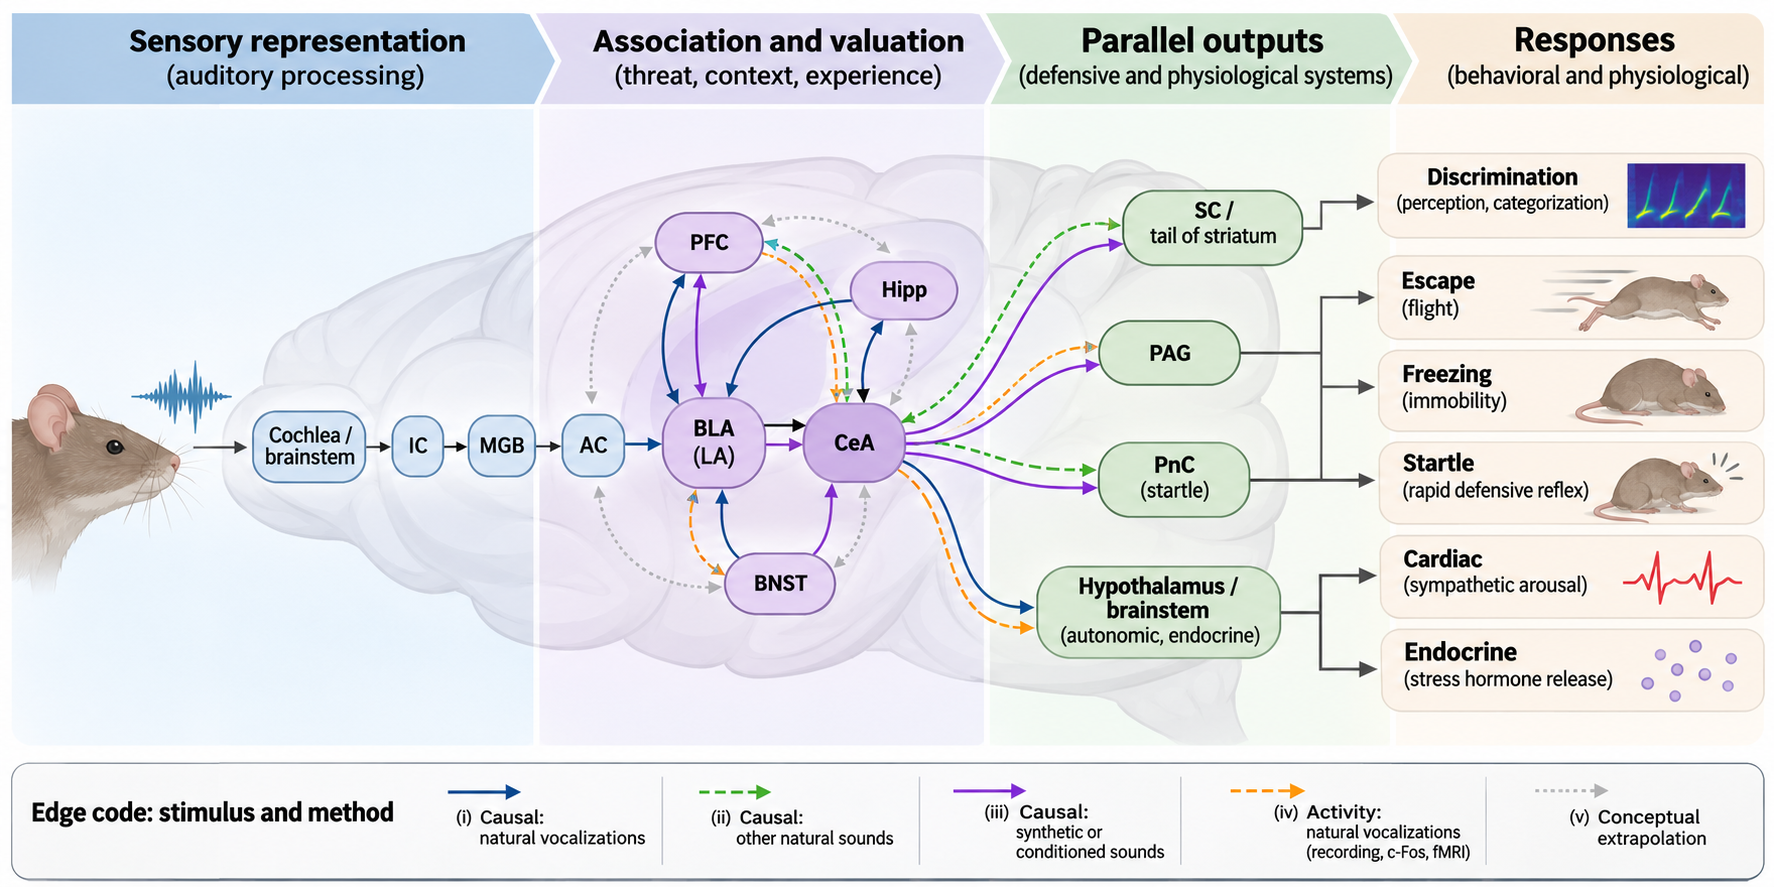
\includegraphics[width=\textwidth]{fig3_ladder_placeholder.png}
  \caption{Parallel pathways from acoustic information to physiological and defensive responses (schematic). Zones: sensory representation (cochlea/brainstem, inferior colliculus, medial geniculate body, auditory cortex); association and valuation (lateral/basolateral and central amygdala, bed nucleus of the stria terminalis, with prefrontal and hippocampal modulation); parallel outputs (periaqueductal gray, acoustic-startle route via caudal pontine reticular nucleus, superior colliculus and tail of striatum, hypothalamic and brainstem autonomic targets); and responses (discrimination, startle, freezing, escape, cardiac and endocrine change). Edges are coded by stimulus and method: (i)~causal evidence with natural vocalizations; (ii)~causal evidence with other natural sounds; (iii)~causal evidence with synthetic or conditioned sounds; (iv)~activity evidence (recording, c-Fos, fMRI) with natural vocalizations; (v)~conceptual extrapolation. Pathways are compiled across preparations; the full network has not been established as a natural alarm-call circuit in any one rodent species.}
  \label{fig:ladder}
\end{figure}

\subsection{Auditory pathways and access to defensive systems}
\label{sec:mechanisms-auditory}

How does a sound reach the parts of the brain that can make an animal afraid? The hearing pathway runs from the cochlea through brainstem nuclei to the inferior colliculus (IC) in the midbrain, then to the auditory thalamus (medial geniculate body, MGB) and auditory cortex. From thalamus and cortex, signals reach the lateral and basolateral amygdala (LA/BLA), the regions most studied when animals learn that a sound predicts danger. Along the way, neurons represent frequency, loudness, and timing. That is feature coding, not meaning. A neuron tuned to 22~kHz can tell call types apart without telling the animal whether the call currently predicts danger.

Classic lesion work in rats established that the thalamus, not the cortex, was needed for a tone paired with shock to raise blood pressure and evoke freezing: auditory cortex lesions left these conditioned responses intact, whereas MGB or IC lesions abolished them \citep{LeDouxEtAl1984}. Recordings later showed that conditioning sharpens short-latency LA responses to the tone \citep{QuirkEtAl1995}. Both studies used conditioned tones. They show that acoustic information can reach the amygdala quickly and that learning reshapes it there. They do not show that cortex is dispensable for sounds with richer structure.

A natural danger cue that is not a call makes the point. A freezing rat falls silent, and the sudden end of its movement sounds can alarm a nearby rat. Freezing to that silence requires the dorsal MGB, a ventral area of auditory cortex, and LA \citep{PereiraEtAl2020}---an ``auditory offset'' pathway that detects the end of a sound rather than its onset. This is causal evidence with another natural sound, not with a vocalization. It shows that a naturalistic cue can depend on both thalamic and cortical stages, unlike the tone in the classic experiments, and it cautions against assuming one obligatory route for every acoustic danger cue.

For natural vocalizations themselves, the evidence at this stage is mostly activity. Amygdala neurons in naïve rats respond differently to 22-kHz and 50-kHz ultrasonic vocalizations (USVs), yet tones matched in frequency reproduce most of that difference, and the rats do not freeze \citep{ParsanaEtAl2012a}. c-Fos mapping after USV playback likewise shows call-type differences in auditory and limbic regions \citep{SadanandaEtAl2008,OudaEtAl2016}, without identifying which regions are required. Sensitivity to frequency or timing is not the same as knowing what a call means.

\subsection{Amygdala circuitry for learned significance and response selection}
\label{sec:mechanisms-amygdala}

Learning that a sound predicts danger and choosing what to do about it are different problems. The amygdala contributes to both, through different components.

The first problem---association---is linked to LA/BLA. In auditory fear conditioning, the tone and the shock converge there, and synaptic inputs from thalamus and cortex are strengthened. Conditioning enhances LA responses to the tone \citep{QuirkEtAl1995} and occludes further potentiation at cortical inputs, as if the synapses had already been strengthened by learning \citep{TsvetkovEtAl2002}. These are causal and cellular findings with conditioned tones. They show how an acoustic association can be stored; they do not tell us how a natural call acquires meaning.

The second problem---selection---is linked to the central amygdala (CeA), which lies closer to output. In mice trained so that a cue shifts from a tone to a burst of white noise, two populations of CeA inhibitory neurons compete: somatostatin-expressing cells promote freezing, corticotropin-releasing-factor-expressing cells promote flight, and each suppresses the other \citep{FadokEtAl2017}. The circuit offers a mechanism for switching rapidly between passive and active defense. It was demonstrated with conditioned sounds, so it is a candidate mechanism for natural calls, not a demonstrated alarm-call pathway. It also shows that even CeA is not a single ``fear center''; competing outputs sit within it.

Rat 22-kHz calls show what experience adds. Rats freeze selectively to a distressed partner's 22-kHz calls only if they have previously experienced shock, and this social transmission of fear requires the auditory thalamus \citep{KimEtAl2010}. The design used a live sender, so multiple cues were available; the causal claim is about thalamic integrity and prior experience, not a complete pathway from LA through CeA. Preventing the receiver from calling during its own shock does not abolish later freezing \citep{CalubEtAl2018}, so hearing oneself call is not required. Meanwhile, naïve rats still slow their heart and locomotion to the same calls \citep{OlszynskiEtAl2020}. Discrimination and bodily response can thus exist without freezing; experience gates the action, not necessarily the perception.

\subsection{Midbrain and brainstem: startle, freezing, and escape}
\label{sec:mechanisms-midbrain}

A sudden noise can make a rodent flinch, freeze, or bolt. These look like points on one scale of alarm, but they arise from at least three distinct families of circuits.

The fastest is the acoustic startle reflex. A short pathway from cochlear root neurons to the caudal pontine reticular nucleus (PnC) in the brainstem, and from there to spinal motor neurons, produces the whole-body flinch within milliseconds \citep{DavisEtAl1982,LeeEtAl1996}. State and learning can modulate startle amplitude, and fear-potentiated startle uses this as a probe of conditioned fear. But a startle shows that a sound was loud and abrupt, not that it was recognized as dangerous.

The second family produces freezing. The periaqueductal gray (PAG) is a midbrain region that organizes defensive movements. In mice, inhibitory projections from CeA to ventrolateral PAG release PAG output neurons, which drive premotor targets in the medulla to produce freezing; this freezing pathway interacts with circuits for flight \citep{TovoteEtAl2016}. The pathway was defined with conditioned sounds and optogenetic manipulation. It explains how a learned acoustic cue can stop an animal in its tracks. It has not been tested for natural calls, or for sciurid vigilance or prairie-dog escape.

The third family drives active escape, and it need not pass through the amygdala at all. Neurons in auditory cortex that project to the IC can trigger flight when activated optogenetically, and silencing them reduces sound-evoked flight; their targets in the IC in turn project to dorsal PAG \citep{XiongEtAl2015}. Sounds that grow louder, mimicking an approaching object, elicit freezing followed by flight in mice: freezing depends on cortical projections to the tail of the striatum, flight on projections to the superior colliculus (SC), and the switch tracks the different time courses of the two targets \citep{LiEtAl2021}. Both studies used synthetic sounds. What they add is architectural: the auditory cortex can drive defense directly, through parallel descending routes, without first assigning learned meaning.

Predatory imminence theory offers a functional frame for these families: animals shift from vigilance to freezing to escape as a threat is judged nearer \citep{Fanselow1994}. The theory organizes defensive priorities. It is not a wiring diagram, and it has not been mapped onto circuits in wild sciurids. Which family a given sound engages depends on the sound, the animal's state, and what the experiment measured (\secref{sec:action}).

\subsection{Autonomic and endocrine channels and extended amygdala}
\label{sec:mechanisms-autonomic}

A sound can change an animal's body without changing its behavior. To see why, it helps to recall how the body's defensive physiology is controlled. The autonomic nervous system has two branches: sympathetic output raises heart rate and blood pressure and mobilizes energy, while parasympathetic output, carried largely by the vagus nerve, slows the heart. The hypothalamic--pituitary--adrenal (HPA) axis acts more slowly: the paraventricular nucleus of the hypothalamus (PVN) triggers a hormonal cascade that ends in glucocorticoid release from the adrenal glands over minutes. Limbic regions, including the amygdala, prefrontal cortex, and hippocampus, shape both systems through relays in the hypothalamus and brainstem, which lets prior experience tune the stress response \citep{UlrichLaiHerman2009}.

These controls run partly in parallel with the motor circuits for defense. In rats given tone--shock conditioning, lesions of the lateral hypothalamus disrupted the conditioned rise in blood pressure but spared freezing, whereas lesions of the midbrain central gray (the PAG) disrupted freezing but spared the blood-pressure response \citep{LeDouxEtAl1988}. Different CeA targets, in other words, carry the cardiovascular and behavioral components of the same learned response. The heart is also a misleading readout on its own. A conditioned tone and an unpaired control tone raised heart rate by the same amount, but by different means: combined sympathetic and parasympathetic drive in conditioned rats, sympathetic drive alone in controls \citep{IwataLeDoux1988}. The same heart rate can hide different physiology.

Direction matters too. Freezing is typically accompanied by a slowing of the heart, a parasympathetic brake that may support attention and preparation for action, whereas flight is accompanied by sympathetic acceleration \citep{Roelofs2017}. Natural calls fit this pattern without settling its mechanism. In rats, 22-kHz calls abruptly lowered heart rate and locomotion, whereas 50-kHz calls raised both, and natural calls had stronger effects than matched tones \citep{OlszynskiEtAl2020}. Juvenile Belding's ground squirrels discriminate alarm call types by heart rate before they discriminate them behaviorally \citep{Mateo1996,Mateo2010}.
% VERIFY: Mateo1996, Mateo2010 (not full-text checked).
Spiny mice raise cortisol to owl calls without detectable freezing or flight, whereas voles show both hormonal and behavioral change \citep{EilamEtAl1999}. These are physiology-and-behavior studies with natural vocalizations; they show what changes, not which pathway changed it.

The bed nucleus of the stria terminalis (BNST), part of the ``extended amygdala,'' is often described as the seat of sustained anxiety. Causal work shows something more specific: BNST is needed for freezing to threat cues that poorly predict when shock will arrive \citep{GoodeEtAl2019}. That suggests a role in uncertainty, which may matter for alarm calls whose reliability varies, but the link has not been tested. During USV playback, BNST- and BLA-related activity differs between 22- and 55-kHz calls in c-Fos and awake fMRI studies \citep{DemaestriEtAl2019,GranataEtAl2024}. This is activity evidence; it locates engagement without establishing necessity.

Autonomic and endocrine change can therefore diverge from behavior because different efferent systems and timescales carry them. That is why a hormone rise is not automatically ``fear,'' why a behavioral null need not mean the sound was ignored, and why a single peripheral measure cannot stand in for an ecological decision. Field physiology has nonetheless relied mainly on glucocorticoids to assess how animals respond to stressors. Heart rate and heart rate variability index sympathetic--adrenal--medullary activation more directly, can complement glucocorticoid measures, and can now be recorded in free-living animals with miniaturized biologgers \citep{GaidicaDantzer2020}. For acoustic risk, that opens a practical bridge between fields: the autonomic dissociations that laboratory studies reveal could be measured in wild receivers as they hear natural calls under realistic costs.

\subsection{Context, learning, and neuromodulatory state}
\label{sec:mechanisms-state}

The same sound does not always mean the same thing. A rat may freeze to a tone in one context and not another; a mother may ignore pup calls before giving birth and run toward them after. Two kinds of mechanism shape this flexibility: forebrain circuits that decide whether a sound matches what was learned, and neuromodulators that set the gain and readiness of the whole system.

Prefrontal cortex and hippocampus help decide how far learned fear should generalize. In rats trained to fear one tone, auditory cortex and the prelimbic region of prefrontal cortex synchronize when a new, safe tone is played, and the strength of that synchrony predicts whether the animal withholds freezing; silencing auditory cortex input to prelimbic cortex, but not to BLA, made rats generalize fear to the new tone \citep{ConcinaEtAl2018}. Dorsal hippocampal lesions had the opposite effect, sharpening discrimination after extensive training \citep{QuinnEtAl2009}. Prefrontal subregions also divide labor: inactivating prelimbic cortex reduced expression of conditioned fear, whereas inactivating infralimbic cortex impaired extinction learning, and ventral hippocampus contributed to both \citep{SierraMercadoEtAl2011}. All of this comes from conditioned tones. It is nonetheless directly relevant to the receiver's problem in the field: whether to treat a new caller or a variant call like a known alarm is a generalization decision.

Neuromodulators adjust how strongly a sound drives behavior. Norepinephrine from the locus coeruleus (LC) helps convert a retrieved auditory fear memory into freezing in conditioned mice \citep{DuanEtAl2025}.
% VERIFY: DuanEtAl2025 stimulus and causal claims against primary text.
Arousal that makes a remembered cue effective is not the same as learning that a particular caller is unreliable. Dopamine shows regional and preparation dependence rather than a threat signal: natural 50-kHz calls transiently raise nucleus accumbens dopamine along with approach, whereas 22-kHz calls do not \citep{WilluhnEtAl2014}, and dopamine responses to noise depend on region, intensity, and whether the noise was predicted, in ways that disagree across preparations \citep{GoedhoopEtAl2022,FuruyamaEtAl2026}. Dopamine is informative about valence and prediction, not a stand-in for alarm-call circuits.

Pup calls offer a revealing non-threat contrast. In mice, oxytocin acting in auditory cortex enables pup-retrieval behavior and rebalances cortical inhibition so that pup calls become more salient \citep{MarlinEtAl2015}. This is causal evidence with natural vocalizations, and it concerns care rather than defense. It shows that neuromodulation can retune how natural calls are heard, and that biologically significant sound is not synonymous with threat.

These mechanisms bridge to the experience- and repetition-dependent updating treated in \secref{sec:persistence}. Generalization, extinction, and neuromodulatory gain are candidate substrates for responses to repeated or unreliable alarms. The circuits that implement caller-reliability updating in wild sciurids remain uncharacterized.

\subsection{What has actually been demonstrated with natural acoustic signals?}
\label{sec:mechanisms-natural}

The circuit map above is impressive. How much of it has been shown for the sounds rodents actually hear in nature? Only part, and the gaps fall in predictable places.

With natural vocalizations, the evidence is strongest for behavior and physiology, weaker for neural activity, and thinnest for causation. Experience-gated freezing to 22-kHz calls, with a causal requirement for the auditory thalamus, is the clearest causal result for a defensive call \citep{KimEtAl2010}. Amygdala recordings and c-Fos maps show call-type differences, some of them stronger for natural calls than for artificial versions matched in frequency and timing \citep{ParsanaEtAl2012a,SadanandaEtAl2008,OudaEtAl2016}. Awake fMRI and c-Fos studies place extended-amygdala engagement during USV playback \citep{DemaestriEtAl2019,GranataEtAl2024}. Autonomic and behavioral measures dissociate across experience and species \citep{OlszynskiEtAl2020,Mateo1996,EilamEtAl1999}. Outside defense, oxytocin-dependent plasticity for pup calls \citep{MarlinEtAl2015} and dopamine responses to 50-kHz calls \citep{WilluhnEtAl2014} show that natural meaning need not be aversive.

With other natural sounds, the evidence is causal but narrow: the thalamic, cortical, and amygdala requirement for freezing to movement-sound cessation \citep{PereiraEtAl2020}.

Field sciurids add a further limit. In Richardson's ground squirrels, chirp and whistle playback produced call-specific c-Fos patterns, including \emph{reduced} labeling in some amygdala and collicular regions relative to no-call controls \citep{FreemanEtAl2020}. Lower c-Fos is not proof of inhibition or of a defensive pathway. The urgency coding, predator-associated categories, and caller reliability documented in marmots, prairie dogs, and ground squirrels (\secref{sec:features}; \secref{sec:action}; \secref{sec:persistence}) pose sharp neural questions that no circuit study has yet addressed.

The causal architecture---CeA competition between freezing and flight, the CeA--PAG freezing pathway, cortical and collicular escape routes, prefrontal control of generalization---comes from synthetic or conditioned sounds \citep{FadokEtAl2017,TovoteEtAl2016,XiongEtAl2015,LiEtAl2021,ConcinaEtAl2018}. None of it has been traced during naturally emitted alarms. Natural acoustic signals have well-documented, context-dependent effects on behavior; the pathways that map them onto valuation, autonomic responses, and ecological action remain far less characterized than those for laboratory threats. That gap is why a comparative field--laboratory perspective is necessary, and \secref{sec:account} uses the circuit evidence to sharpen what the field comparisons predict.
